\tikzsetnextfilename{setup}
\begin{center}
   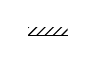
\begin{tikzpicture}

      \usetikzlibrary{patterns}
      % We define a tikz style which defines a fill pattern consisting of lines in the north east direction.
      % The draw=none option indicates that we do NOT want any stroke/border around the fill
      \tikzstyle{wall}=[fill,pattern=north east lines,minimum width=0.75cm,minimum height=0.3cm, draw=none]

      \def\hw{0.25}     % Half width of the small wall segment on top

      \draw (-\hw, 0) -- (\hw, 0);
      \draw [wall] (-\hw,0) rectangle (\hw,0.1);        % Draws a rectangle using the 'wall' pattern giving us the sloped lines


   \end{tikzpicture}
\end{center}
